\section{PHP}
\subsection{Bedeutung PHP}

PHP ist eine Open-Source-Skriptsprache 
f"ur den allgemeinen Gebrauch, 
die speziell f"ur die Webprogrammierung entwickelt wurde 
und in HTML integriert werden kann. 
 PHP zeichnet sich von clientseitigen Sprachen
  wie Javascript dadurch aus, 
  dass der Code auf dem Server ausgef"uhrt wird, 
  wo er eine HTML-Ausgabe erzeugt, 
  die an den Kunde geschickt wird. 
  Der Kunde bekommt daher nur das Ergebnis der Skriptausf"uhrung, 
  ohne wissen zu k"onnen, wie der tats"achliche Code aussieht. 
  Es besteht  die M"oglichkeit, 
  dass Ihr Webserver alle Ihre HTML-Dateien mit PHP pr"uft, 
  weil es dann wirklich nichts gibt, 
  was man dem Benutzer sagen kann, was es in petto enth"alt.

Das Besondere an der Benutzung von PHP ist, 
dass es f"ur Anf"anger extrem einfach zu bedienen ist,
 aber auch eine Vielzahl von Funktionen f"ur den 
 professionellen Programmierer bietet.  
 Die lange Liste der PHP-Funktionen zu lesen,macht kein Problem.
 Weil es m"oglich ist,
 in weniger Stunden einfache Skripten zu erstellen[25].

\subsection{Hauptgebiete der PHP-Skripte}

Es gibt drei Hauptbereiche, in denen PHP-Skripte verwendet werden :
\begin{itemize}
\item Serverseitige Programmierung. 
Dies ist die traditionelle und das wichtigste Bereich 
von PHP. Es braucht drei Dinge,
 um es zu benutzen: 
 Der PHP-Parser (CGI\footnote{CGI bedeutet allgemein Verwaltungsrechner Schnittstelle} oder Servermodul), 
 ein Webserver und ein Webbrowser. Es muss einen Webserver 
 ausgef"uhrt werden, der mit einer PHP-Installation verbunden ist. 
 Es ist m"oglich, auf die Ergebnisse des PHP-Programms 
 "uber einen Webbrowser zu reagieren, 
 der die Seite "uber den Server anzeigt. 
 Es kann all dieses Skript auf Ihrem PC ausgef"uhrt werden, 
 wenn man zuerst mit der PHP-Programmierung ausprobieren will.
 
 
\item Befehlszeilenprogrammierung. 
Es ist ebenfalls m"oglich, PHP-Skripte zu schreiben, 
die ohne Server oder Browser funktionieren. 
Alles, was es ben"otigt ist, ist der PHP-Parser. 
Die Nutzungsart ist ideal f"ur Programme, 
die h"aufig mit cron (unter Linux) oder (unter Windows) 
durchgef"uhrt werden. 
Skripte k"onnen auch f"ur 
eine einfache Textverarbeitung verwendet werden.



\item Schreiben von Desktop-Applikationen. 
PHP ist wahrscheinlich nicht die allerbeste Sprache, 
um Desktop-Anwendungen mit grafischer Oberfl"ache zu schreiben, 
aber wenn Sie PHP sehr gut kennen und einige weiterf"uhrende 
PHP-Features in Ihren clientseitigen Applikationen nutzen m"ochten, 
k"onnen Sie PHP-GTK nutzen, um derartige Programme zu schreiben. 
Auf diese Art haben Sie auch die M"oglichkeit, 
plattform"ubergreifende Applikationen zu schreiben. 
PHP-GTK\footnote{GTK bedeutet in dieser Arbeit ein Paket von Sprachverbindungen f"ur PHP} ist eine Erweiterung von PHP, 
die in der Hauptdistribution nicht enthalten ist.
\end{itemize}

PHP kann auf allen wichtigen Betriebssystemen genutzt werden, 
einschließlich Linux, 
vielen Unix-Varianten (einschlie"slich HP-UX, Solaris und OpenBSD), 
Microsoft Windows, MacOS, RISC OS und möglicherweise anderen. 
PHP ist auch kompatibel mit den meisten aktuellsten Webservern. 
Dazu gehören Apache, Microsoft Internet Information Server, 
Personal Web Server, Netscape und iPlanet Server, 
Oreilly Website Pro Server, Caudium, Xitami, 
OmniHTTPd und viele andere. 
F"ur die meisten Server stellt PHP ein eigenes Modul zur Verf"ugung, 
f"ur andere, die den CGI-Standard erf"ullen, 
kann PHP als CGI-Prozessor eingesetzt werden[26]. 
%
\subsection{Warum PHP?}

PHP ist die am h"aufigsten verwendete Programmiersprache und die Sprache 
f"ur die Entwicklung dynamischer Webanwendungen,
weil es einfach funktioniert.
Die PHP-Programmierung kann alles tun, 
was eine andere Programmiersprache 
f"ur dynamische Anwendungen tun kann.
Der Vergleich von Programmiersprachen ist schwierig, 
da jede ihre Vor- und Nachteile hat. Grunds"atzlich ist 
jedoch die Aussage, dass PHP einfach und schnell ist. 
Die Nachteile von PHP sind erh"ohrter Netzwerktraffic,
Gerschwindigkeitsnachteil beim Kompilieren des Skriptes[38].
Experten zufolge ist die Syntax von PHP der von ASP 
 und JSP "uberlegen und leistungsf"ahiger als ColdFusion und viel 
einfacher zu erlernen als Pearl. Diese Vorteile machen PHP 
zur am weitesten verbreiteten Programmiersprache[27].

\subsection{Datenbank}

Die effiziente Speicherung und Abfrage gro"ser Datenmengen hat wesentlich 
zum Erfolg des Internets beigetragen, das in der Regel 
mit Hilfe von Datenbanken realisiert wird: Seiten wie Yahoo, Amazon 
und Ebay sind stark von der Zuverl"assigkeit von Datenbanken abh"angig, 
in denen gro"se Mengen an Informationen gespeichert sind.
Der Datenbank-Support ist jedoch nicht im Web, 
f"ur den Webentwickler reserviert, verschiedene leistungsstarke 
Implementierungen werden zu relativ niedrigen Preisen 
(oder sogar kostenlos) angeboten, 
das Hinzuf"ugen von Such- und Sortierfunktionen auf Ihrer 
Website ist viel einfacher, und die Steuerung von Berechtigungen 
ist dank der Berechtigungskontrollfunktionen 
vieler Datenbanksysteme einfach[28].

\subsection{Definition von SQL}

SQL k"onnte kurz als Standardsprache f"ur die Interaktion mit 
relationalen Datenbanken beschrieben werden. 
SQL ist aber keine Computersprache wie C, C++ oder PHP. 
Es ist vielmehr ein Interface-Tool, 
mit dem man verschiedene Befehle ausf"uhren kann. 
SQL ist jedoch nicht nur eine Abfragesprache (wie der Name schon sagt), 
sondern bietet eine Vielzahl von Werkzeugen f"ur die Datenbankinteraktion:

\begin{itemize}
\item Datenstrukturdefinition: SQL kann die verschiedenen Konstruktionen 
definieren, die die Datenbank zum Speichern von Daten verwendet.
\item Datenabfrage: SQL kann Daten aus einer Datenbank abrufen 
und in einem einfach zu lesenden Format anzeigen.
\item Datenbearbeitung: SQL kann Daten einf"ugen, 
aktualisieren und aus der Datenbank l"oschen.
\item Datenzugriffskontrolle: SQL kann verwendet werden, um zu steuern,
 wer Daten basierend auf dem Benutzer anzeigen, einf"ugen, 
 aktualisieren und l"oschen darf.
 \item Datenintegrit"at: SQL verhindert Datenverluste aufgrund paralleler 
 Datenaktualisierungen oder Systemausf"alle[28].
 



Nach der Definition ist SQL besonders f"ur relationale Datenbanken bestimmt. 
Eine analytische Datenbank ist eine Datenbankimplementierung, 
bei der alle Daten in Tabellen mit einem einzigartigen Namen 
untergliedert sind. Es kann eine Tabelle in Form von Datenwerten wie beschrieben in Abbildung~\ref{fig:Daten}
aufgebaut werden, bei der die Position der Daten pro Zeile/Spalte 
definiert wird. Dieses Format wird in der Regel 
auch f"ur die Darstellung verwendet[28].
 

 \end{itemize}
 \begin{figure}[!htb]
\begin{center}
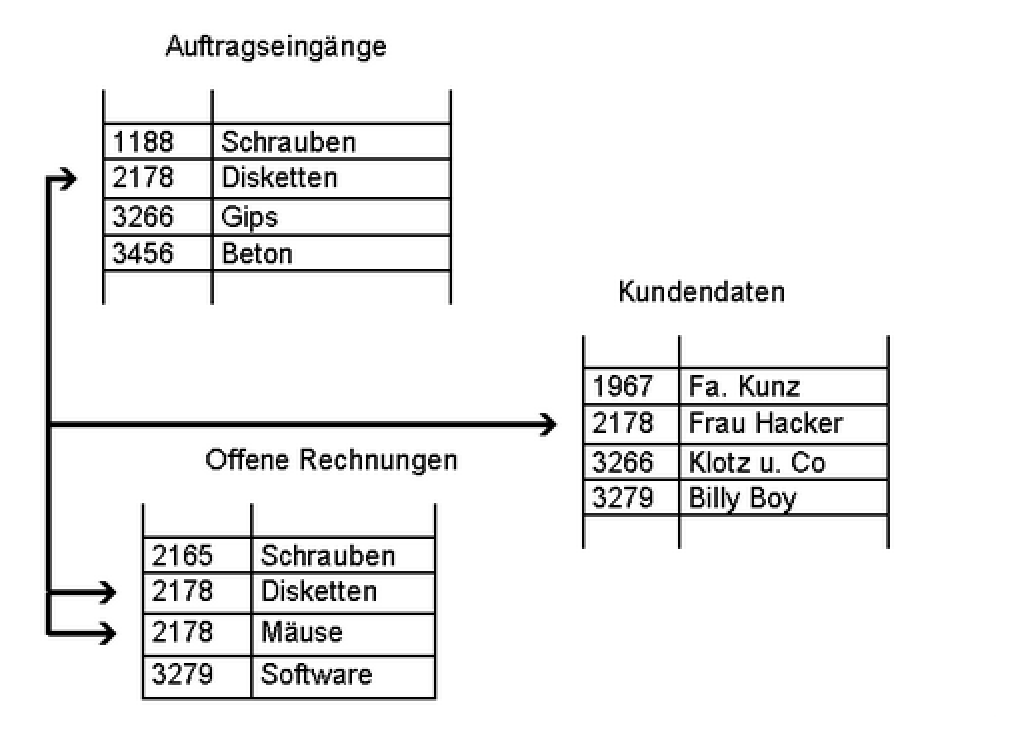
\includegraphics[height=6cm]{bilder/Daten.eps}
\end{center}
\caption{Beispiel einer relationalen Datenbank[29]}\label{fig:Daten}
\end{figure}




\subsection{was ist MySQL?}

MySQL ist ein zuverl"assiger SQL-Datenbank-Server, 
der von T.c.X DataKonsultAB in Stockholm, Schweden, entwickelt wurde[30]. 
Seit der Entwicklung im Jahr 1995 hat sich MySQL zu einem der 
beliebtesten Datenbankserver der Welt etabliert. 
Diese Akzeptanz ist zum Teil auf die Schnelligkeit, 
Stabilit"at und Flexibilit"at der Lizenzpolitik von MySQL zur"uckzuf"uhren, 
die im Vergleich zu PHP aufgrund ihrer Funktionen und vieler 
vordefinierter und einfach zu bedienender Schnittstellenfunktionen 
eindeutig die beliebteste Datenbank geworden ist[28].
MySQL organisiert, stellt dar, bewahrt und modifiziert 
Daten der klassischen Aufgabe 
eines Datenbank-Managementsystems.
Es arbeitet als Client-Server-System: Die entsprechende Datenbank ist der Server.
 Die clientseitige Software sendet Befehle an die Datenbank. 
 Die Datenbank wandelt die Auftr"age in vollziehbaren Code um, 
 f"uhrt die Auftr"age aus und schickt die Informationen "uber sie an den Kunden[28][30].
 
\subsection{Serielle Communication}

Die Universal Asynchronous Transmitter Software Library (UART) wird 
f"ur die RS232-basierte serielle Kommunikation zwischen zwei 
elektronischen Geräten verwendet. Bei der seriellen Kommunikation werden 
nur zwei Kabel ben"otigt, um Daten in beide Richtungen zu "ubertragen. 
Die Daten werden im seriellen Format an den Logikpin1, auch bekannt als Mark, 
gesendet. Die Daten"ubertragung beginnt, wenn dieser Pin auf Logik 0,
 auch bekannt als SPACE, wechselt. Das letzte gesendete Bit ist das 
 Stopp bit mit Logik 1. Serielle Daten werden in der Regel als 10-Bit-Frame gesendet, 
 der sich aus einem Startbit, 8 Daba-Bits und einem Stoppbit und keinem Priorit"atsbit zusammensetzt.
Die Abbildung~\ref{fig:AS} zeigt, wie das Zeichen A "uber die serielle Kommunikation 
gesendet werden kann. Zeichen A hat das Bin"armodell ASCII 01000001,
 wie in der Abbildung dargestellt, das Startbit wird zuerst gesendet, 
 gefolgt von 8 Datenbits 01000001, und schließlich wird das Stoppbit  gesendet.




\begin{figure}[!htb]
\begin{center}
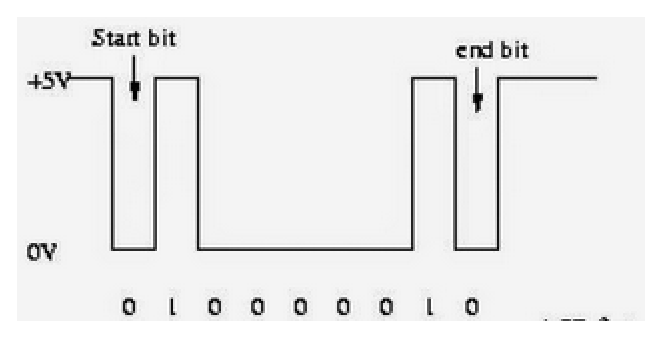
\includegraphics[height=6cm]{bilder/AS.eps}
\end{center}
\caption{Sendung der Character A in Serial Communication[40]}\label{fig:AS}
\end{figure}



Die Bit-Timings sind bei der seriellen Kommunikation sehr wichtig, 
und der Sender (TX) und der Empf"anger (RX) m"ussen die gleichen Bit-Timings 
haben. Das Bit-Timing wird durch die Baudrate gemessen, die die Anzahl 
der "ubertragenen oder empfangenen Baudraten pro Sekunde angibt. 
Typische Baudraten sind 4800,9600,19200,19200,38400 usw. 
Beispielsweise werden bei einem Betrieb mit 9600 Baudrate mit einer 
Bildgr"o"se von 10 Bit pro Sekunde 960 Zeichen gesendet oder empfangen. 
Das Timing zwischen den Bits betr"agt dann etwa 104ms[40]. 















